\documentclass[sigconf, 9pt]{acmart}


\usepackage{xcolor}

\usepackage{float}
\usepackage{siunitx}


\newif\iffinal

% \finaltrue

\iffinal
  \newcommand{\tyler}[1]{}
  \newcommand{\ian}[1]{}
  \newcommand{\kyle}[1]{}
\else
  \newcommand{\tyler}[1]{{\textcolor{cyan}{ tyler: #1 }}}
  \newcommand{\ian}[1]{{\textcolor{red}{ Ian: #1 }}}
  \newcommand{\kyle}[1]{{\textcolor{purple}{ Kyle: #1 }}}
\fi


%%
%% \BibTeX command to typeset BibTeX logo in the docs
\AtBeginDocument{%
  \providecommand\BibTeX{{%
    \normalfont B\kern-0.5em{\scshape i\kern-0.25em b}\kern-0.8em\TeX}}}


\newcommand{\name}{Xtract}
\newcommand{\funcx}{$f$\kern-0.18em\emph{unc}\kern-0.05em X}

\acmConference{Fifth International Workshop on Serverless Computing (WoSC)}{2019}{Davis, CA}

\begin{document}


\title{Harnessing Serverless to Extract File Metadata at the Edge}


\author{Tyler J. Skluzacek} 
\affiliation{University of Chicago}
\email{skluzacek@uchicago.edu}



\renewcommand{\shortauthors}{Skluzacek et al.}

\begin{abstract}

The rapid generation of data from distributed IoT devices, scientific instruments, and compute clusters presents
unique challenges in data management. The influx of massive, increasingly-complex data causes repositories to become 
siloed or generally unsearchable---both problems not currently well-addressed by distributed file systems.  
In this work we propose \name{}, a serverless middleware 
to extract inscribed metadata from files across heterogeneous edge computing resources. Moreover, we intend to study how \name{} can
automatically construct file extraction workflows subject to users' cost, time, compute allocation preference, and security constraints. 
To this end, \name{} creates a searchable centralized index across distributed data collections.


\end{abstract}

\begin{CCSXML}
<ccs2012>
<concept>
<concept_id>10002951.10003227.10010926</concept_id>
<concept_desc>Information systems~Computing platforms</concept_desc>
<concept_significance>500</concept_significance>
</concept>
<concept>
<concept_id>10002951.10003317.10003365.10003366</concept_id>
<concept_desc>Information systems~Search engine indexing</concept_desc>
<concept_significance>300</concept_significance>
</concept>
<concept>
<concept_id>10010405.10010497.10010500.10010503</concept_id>
<concept_desc>Applied computing~Document metadata</concept_desc>
<concept_significance>500</concept_significance>
</concept>
</ccs2012>
\end{CCSXML}

\ccsdesc[500]{Information systems~Computing platforms}
\ccsdesc[500]{Applied computing~Document metadata}
\ccsdesc[300]{Information systems~Search engine indexing}

\keywords{data lakes, serverless, metadata extraction, file systems}

\maketitle


\section{Introduction}

The rapid generation of data from IoT devices, scientific instruments, and personal computing devices presents unique 
data management challenges. Currently data are spread across multiple machines, are generally siloed, and require 
significant manual labor by users to create metadata that make the data on these devices searchable. Some~\cite{egan2003vizier, welter2013nhgri, irods, dataverse}  have created data catalogs from user-submitted metadata. These, however, are not scalable to current and future storage systems,
as humans cannot possibly label billions of heterogeneous files.   
In order to build a global metadata catalog over distributed big data, we require automated methods to crawl data, extract 
metadata attributes for each file, and populate a global search index for users to find and access data. Others have developed end-to-end 
automated metadata extraction systems, but they require that data be moved to a central service~\cite{skluzacek2018skluma, skluzacek2016klimatic, padhy2015brown, rodrigo2018sciencesearch} or do not have built-in scaling capabilities~\cite{mattmann2011tika}. 
In this work we strive to create a scalable, decentralized metadata extraction system that eschews the need to send files to a central service.  

We present our prototype and vision for \name{},
a serverless middleware that provides high-throughput and on-demand metadata 
extraction, enabling the automated creation of rich, searchable data lakes from previously unsearchable data swamps. 
Serverless computing, and specifically function as a service (FaaS),
provides an ideal model for managing the invocation of
many short-running extractors on an arbitrarily large number of files. 
\name{} uses the \funcx{} serverless supercomputing platform~\cite{chard2019serverless}
to execute functions across diverse and distributed computing infrastructure.
%We propose the use of FaaS for mapping the metadata extraction problem to a 
%collection of granular metadata extractor functions. 
%We describe how such a model can support the flexibility, scalability, and extensibility required
%for scientific metadata extraction. 
Rather than rely on commercial FaaS systems, we explore a novel distributed FaaS model 
that overcomes the limitation of moving large amounts of data to the cloud. 
Instead, we are able to push
metadata extractors to the edge systems on which the scientific data reside. 
The contributions of \name{} are the following: 
%\name{} is advantageous to existing metadata extraction systems in that it: 
\begin{itemize}
\item Infinitely scalable across all user resources, from IoT to clouds and clusters. 
\item Deploys endpoints at data, enabling decentralized data processing. 
\item Dynamically constructs unique metadata extractor pipelines for diverse file types. 
\item Intelligently makes data staging decisions based on user-supplied constraints. 
\item Automatically populates a search index of rich, searchable metadata. 
\end{itemize}

%\kyle{I'd like to see more about the novelty of the assembled pipelines in this list}


%The remainder of this paper is organized as follows. 
%\S\ref{sec:approach} presents our proposed architecture for \name{}. 
%\S\ref{sec:eval} discusses metrics and workloads used to evaluate its performance. 
%Finally, \S\ref{sec:conc} contains concluding remarks.


\section{Approach}
\label{sec:approach}

\name{} will exist as a serverless metadata extraction middleware that runs atop the \funcx{} serverless 
computing platform, allowing users to optimize metadata extraction workflows subject to 
extraction time, cost, available compute allocations, and security policies.
The \name{} architecture is shown in Figure~\ref{fig:arch}.
The remainder 
of this section outlines the existing \name{} prototype, and imminent goals for it. 

\textbf{Metadata extractors} are functions that input a file or group of files, and output a metadata dictionary. 
Each metadata extractor runs in a given container runtime with all required dependencies (i.e., files and 
libraries).  Our system currently provides a number of built-in extractors, including
those to extract metadata from tabular, structured JSON/XML data, free text, and images. In future we work, 
we plan to support user-submitted metadata extractors, automatically generate runtimes based on inferred 
dependency requirements, and also train \name{} to recognize when a user-submitted extractor 
is appropriate for an arbitrary file. 

The \textbf{\name{} service} prototype dynamically applies a set of metadata extractors to files. 
It does so by constructing a dynamic extractor workflow for each file 
or group of files in a repository.  
First, \name{} sends a crawler function to endpoints specified by the user.  The crawler creates an 
initial metadata dictionary for each file by finding physical properties (e.g., path, size, extension, hash) of each file or group of files
in a given data set.  Once the initial dictionary is created, \name{} invokes a file type extractor on each file that determines probable downstream extractors for each file. We've shown in past work~\cite{skluzacek2018skluma} that feeding the first 512 bytes of a file into 
a trained random forests model can predict a file's type with accuracy higher than the Unix `file' command (due to lack of information in `magic' bytes) and in less time
than attempting to execute incorrect extractors on each file. Once file type is determined the extractor executes the remaining library of extractors 
on each file by sending extractor functions to the endpoint, and sending additional extractors based on the returned metadata.  For instance, 
a tabular data file with multiple lines of free text header (e.g., describing experimental setup) may be identified by the system as a tabular file, but 
the metadata from the tabular 
extractor will state the lines of the file that may be eligible for processing by a free text extractor (e.g., extract keywords from it).
Requests to the web service are protected using Globus Auth~\cite{tuecke2016globus}, and all resulting metadata are stored to a searchable Globus Search index. 

\funcx{} \textbf{endpoints} can currently be deployed across myriad compute providers, from personal computing devices (i.e., laptops), compatible 
IoT devices, cloud providers, and HPC systems.  Endpoints build upon the Parsl~\cite{babuji2019parsl} parallel programming library to 
provision compute resources on a given system, and to manage the execution of functions in containers on said resources. \funcx{} enables 
\name{} to execute metadata extraction functions at any registered and accessible \funcx{} endpoint.  \funcx{} enables \name{} to reliably 
scale to thousands of nodes and simultaneously deploy metadata extraction tasks on arbitrary compute resources. 
\funcx{} supports Singularity and Shifter, allowing \name{} extractors to be executed
on various high performance computing systems. 



\begin{figure}[t]
	\centering
	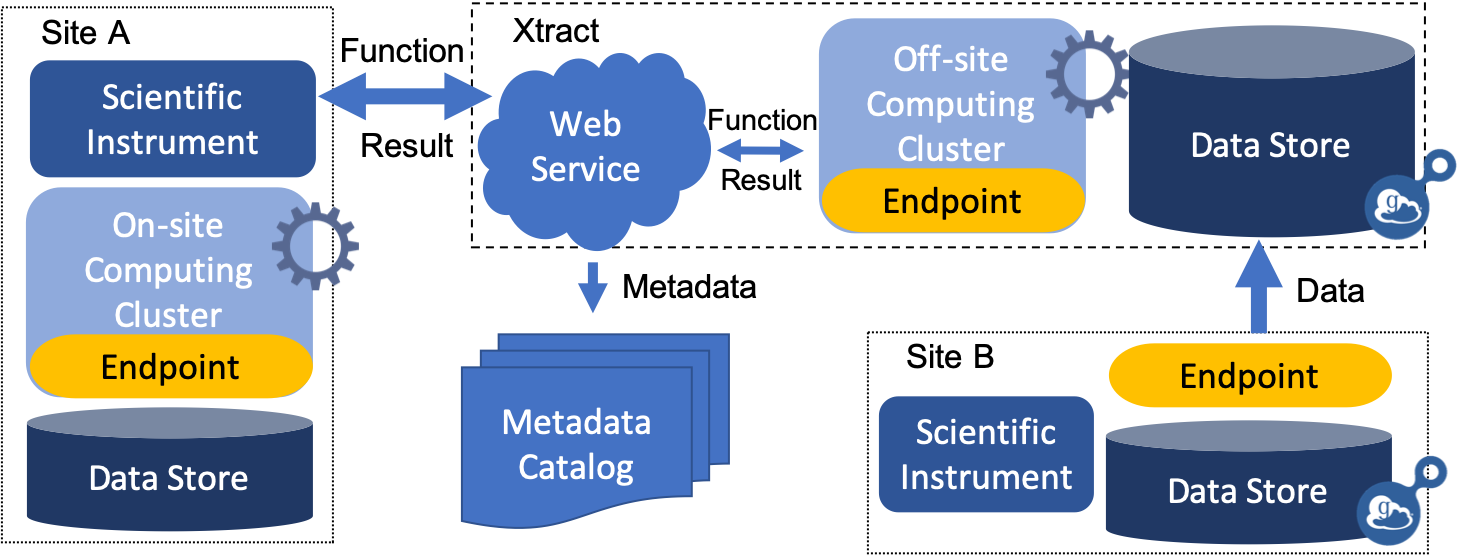
\includegraphics[scale=0.17]{figs/updated-fig.png}
	\caption{Overview of the \name{} architecture. For \textit{Site A} functions are transmitted to the remote resource and performed on local computing resources, returning metadata to the \name{} service. \textit{Site B} lacks suitable local
	computing capabilities, requiring data to be staged to \name{} for analysis.}
	\label{fig:arch}
\end{figure}


\section{Evaluation Plan}
\label{sec:eval}

In future work we plan to study how \name{} can self-optimize subject to real-world, user-defined constraints for heterogeneous data stored across multiple 
endpoints.  Specifically, we plan to explore how augmenting metadata extraction workflows to stage data to idle or under-utilized resources could 
find a globally optimal computing continuum with respect to user constraints of financial cost, computing time, desired compute usage on 
given resource allocations, and security. 

We intend to evaluate \name{}'s self-optimization strategies subject to a large number of constraint combinations across diversity of datasets. 
These include the Carbon Dioxide Information Analysis Center (330+ GB, 10,000 
unique file extensions of carbon dioxide data), the Materials Data Facility~\cite{ blaiszik2019mdf} (30+ TB, tens of millions of materials science files); 
Petrel (4+ PB, 50,000+ files of cross-disciplinary data at Argonne National Lab), and Globus (over 20,000 unique, connected 
endpoints containing hundreds of billions of files).


\section{Conclusion}
\label{sec:conc}

\name{} enables users to support the search and organization of large, distributed data sets by dynamically constructing metadata extraction 
workflows for each file. \name{} is a serverless middleware that solves the data locality and scalability challenges by deploying compute endpoints on the data's native edge
devices and constructing extraction workflows subject to a number of user constraints. Such a system will enable companies, researchers, and individuals alike to more easily find, understand, and share increasingly 
complex data sets, leading to enhanced scientific and industrial progress. 


\begin{acks}

This research is conducted under the guidance of Dr. Ian Foster and Dr. Kyle Chard, and with contributions
from Dr. Ryan Chard, Dr. Zhuozhao Li, Yadu Babuji, and Ryan Wong. 


\end{acks}
\bibliographystyle{ACM-Reference-Format}
\bibliography{wosc}


\end{document}
\endinput
